\section{The vorticity equation}\label{the-vorticity-equation}

\subsection{Western intensification}\label{western-intensification}

It is interesting to analyze the meridional vorticity flux

\[\zeta v = \left( \frac{\partial v}{\partial x} -\frac{\partial u}{\partial y}\right) v = \frac{1}{2}\frac{\partial }{\partial x} v^2 -\frac{\partial }{\partial y} u v + u \frac{\partial v}{\partial y}\]

but using the continuity equation \(u_x+v_y=0\), we obtain

\[\zeta v = \frac{1}{2}\frac{\partial }{\partial x} v^2 -\frac{\partial }{\partial y} u v -u \frac{\partial u}{\partial x}= -\frac{\partial }{\partial y} u v -\frac{1}{2}\frac{\partial }{\partial x}( u^2-v^2)\]

similarly we get

\[\zeta u =  \frac{\partial }{\partial x} u v -\frac{1}{2}\frac{\partial }{\partial y}( u^2-v^2)\]

It is interesting to look at the average flux over a domain bounded in
longitude and latitude, like for instance an ocean basin as it is shown
in Fig. \texttt{fig:1}. Boundary conditions are imposed so that zonal
velocities are zero at east and west walls, as the meridional velocity
is zero a t the north and south walls. The total value of the vorticity
flux over the region is therefore

\begin{figure}
\centering
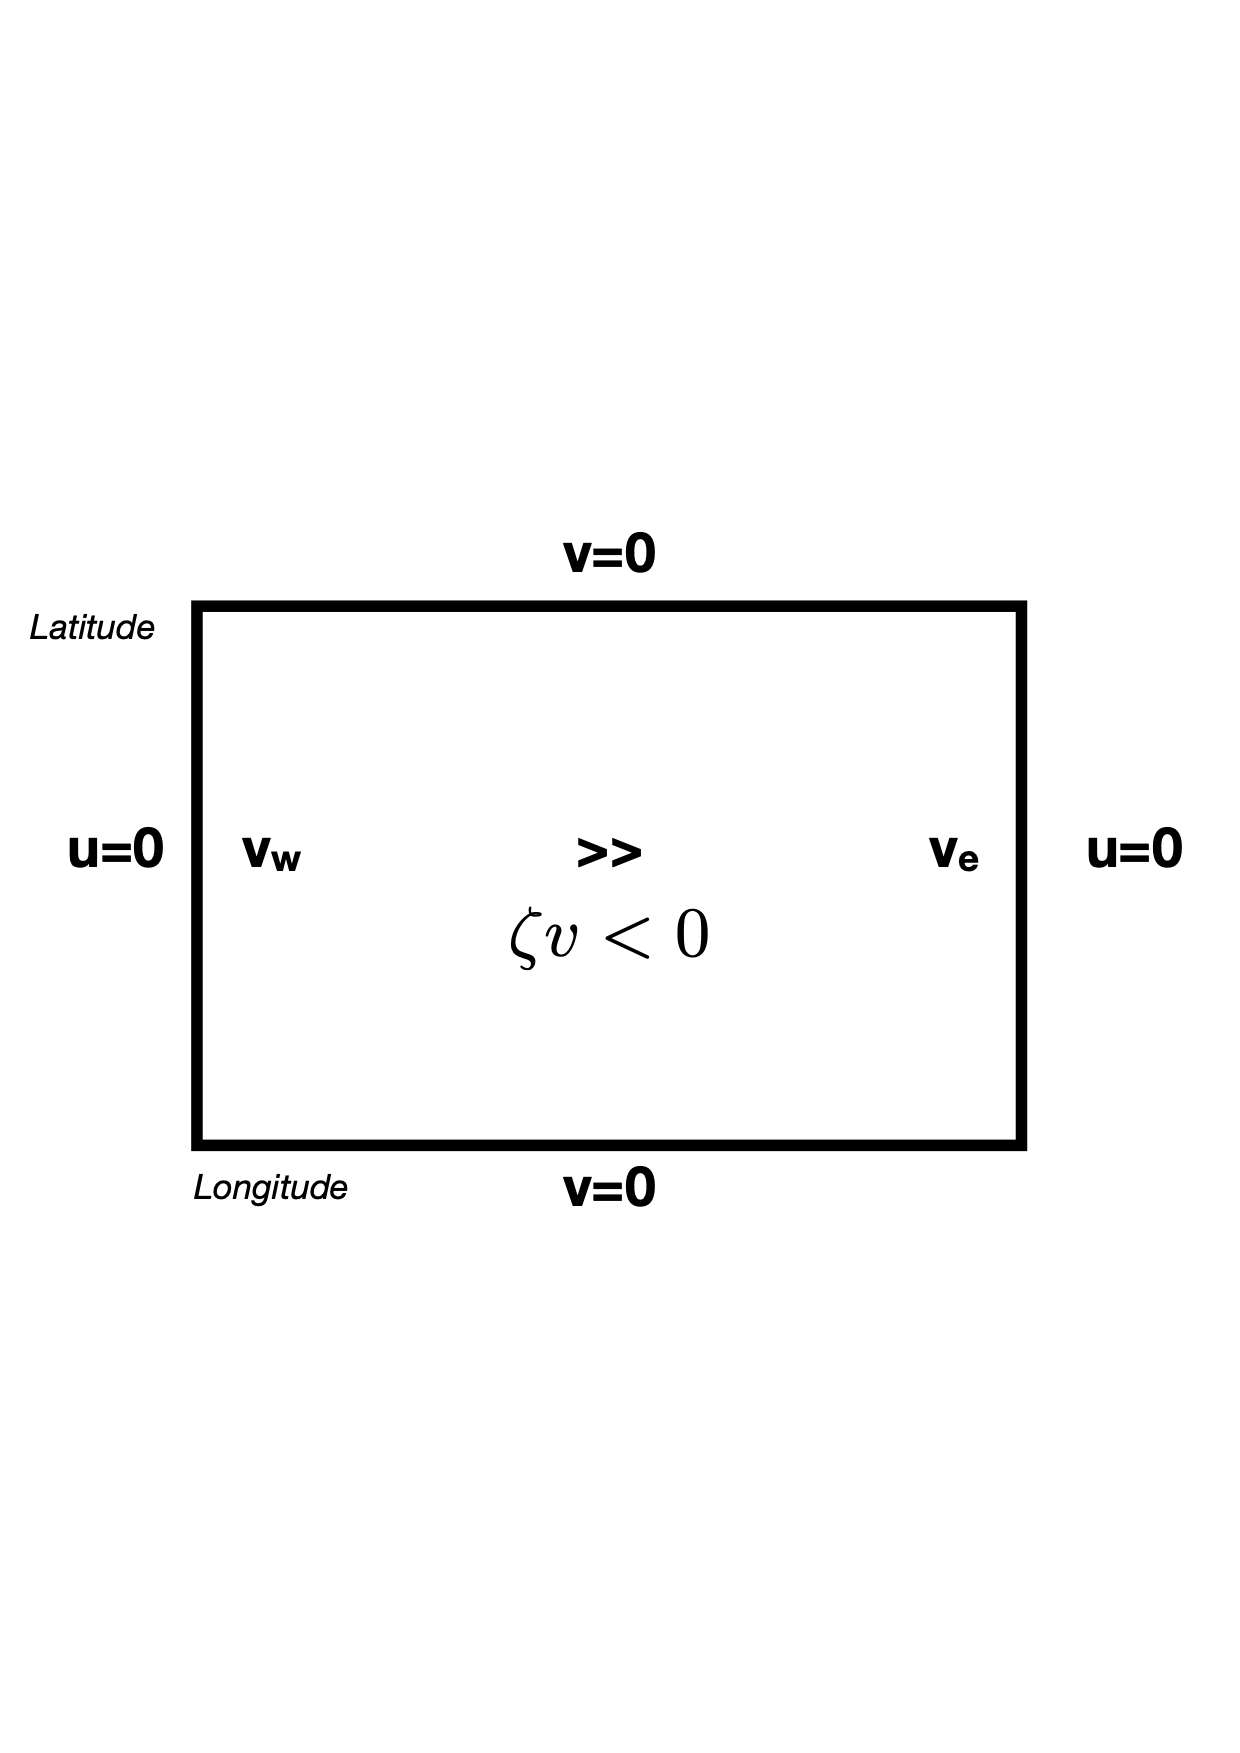
\includegraphics[width= .7 \textwidth]{figs/GD/Untitled.png}
\caption{}
\label{fig:}
\end{figure}

\[\int\int \, \zeta v dx dy = -\int dy \frac{1}{2}\left.(u^2-v^2)\right|^{East}_{West}=\int dy \frac{1}{2}\left( v^2_{East}-v^2_{West}\right)\]

so a negative vorticity flux (i.e. equatorward) is necessary for
meridional velocities to be larger at the western boundary. This is the
basic mechanism for the western intensification of currents in limited
basin over a rotating planets, namely the mechanism that creates the
Gulf Stream and the Kuroshio currents.

The spherical geometry of the Earth also suggests another case, the
Polar cap.


\begin{figure}
\centering
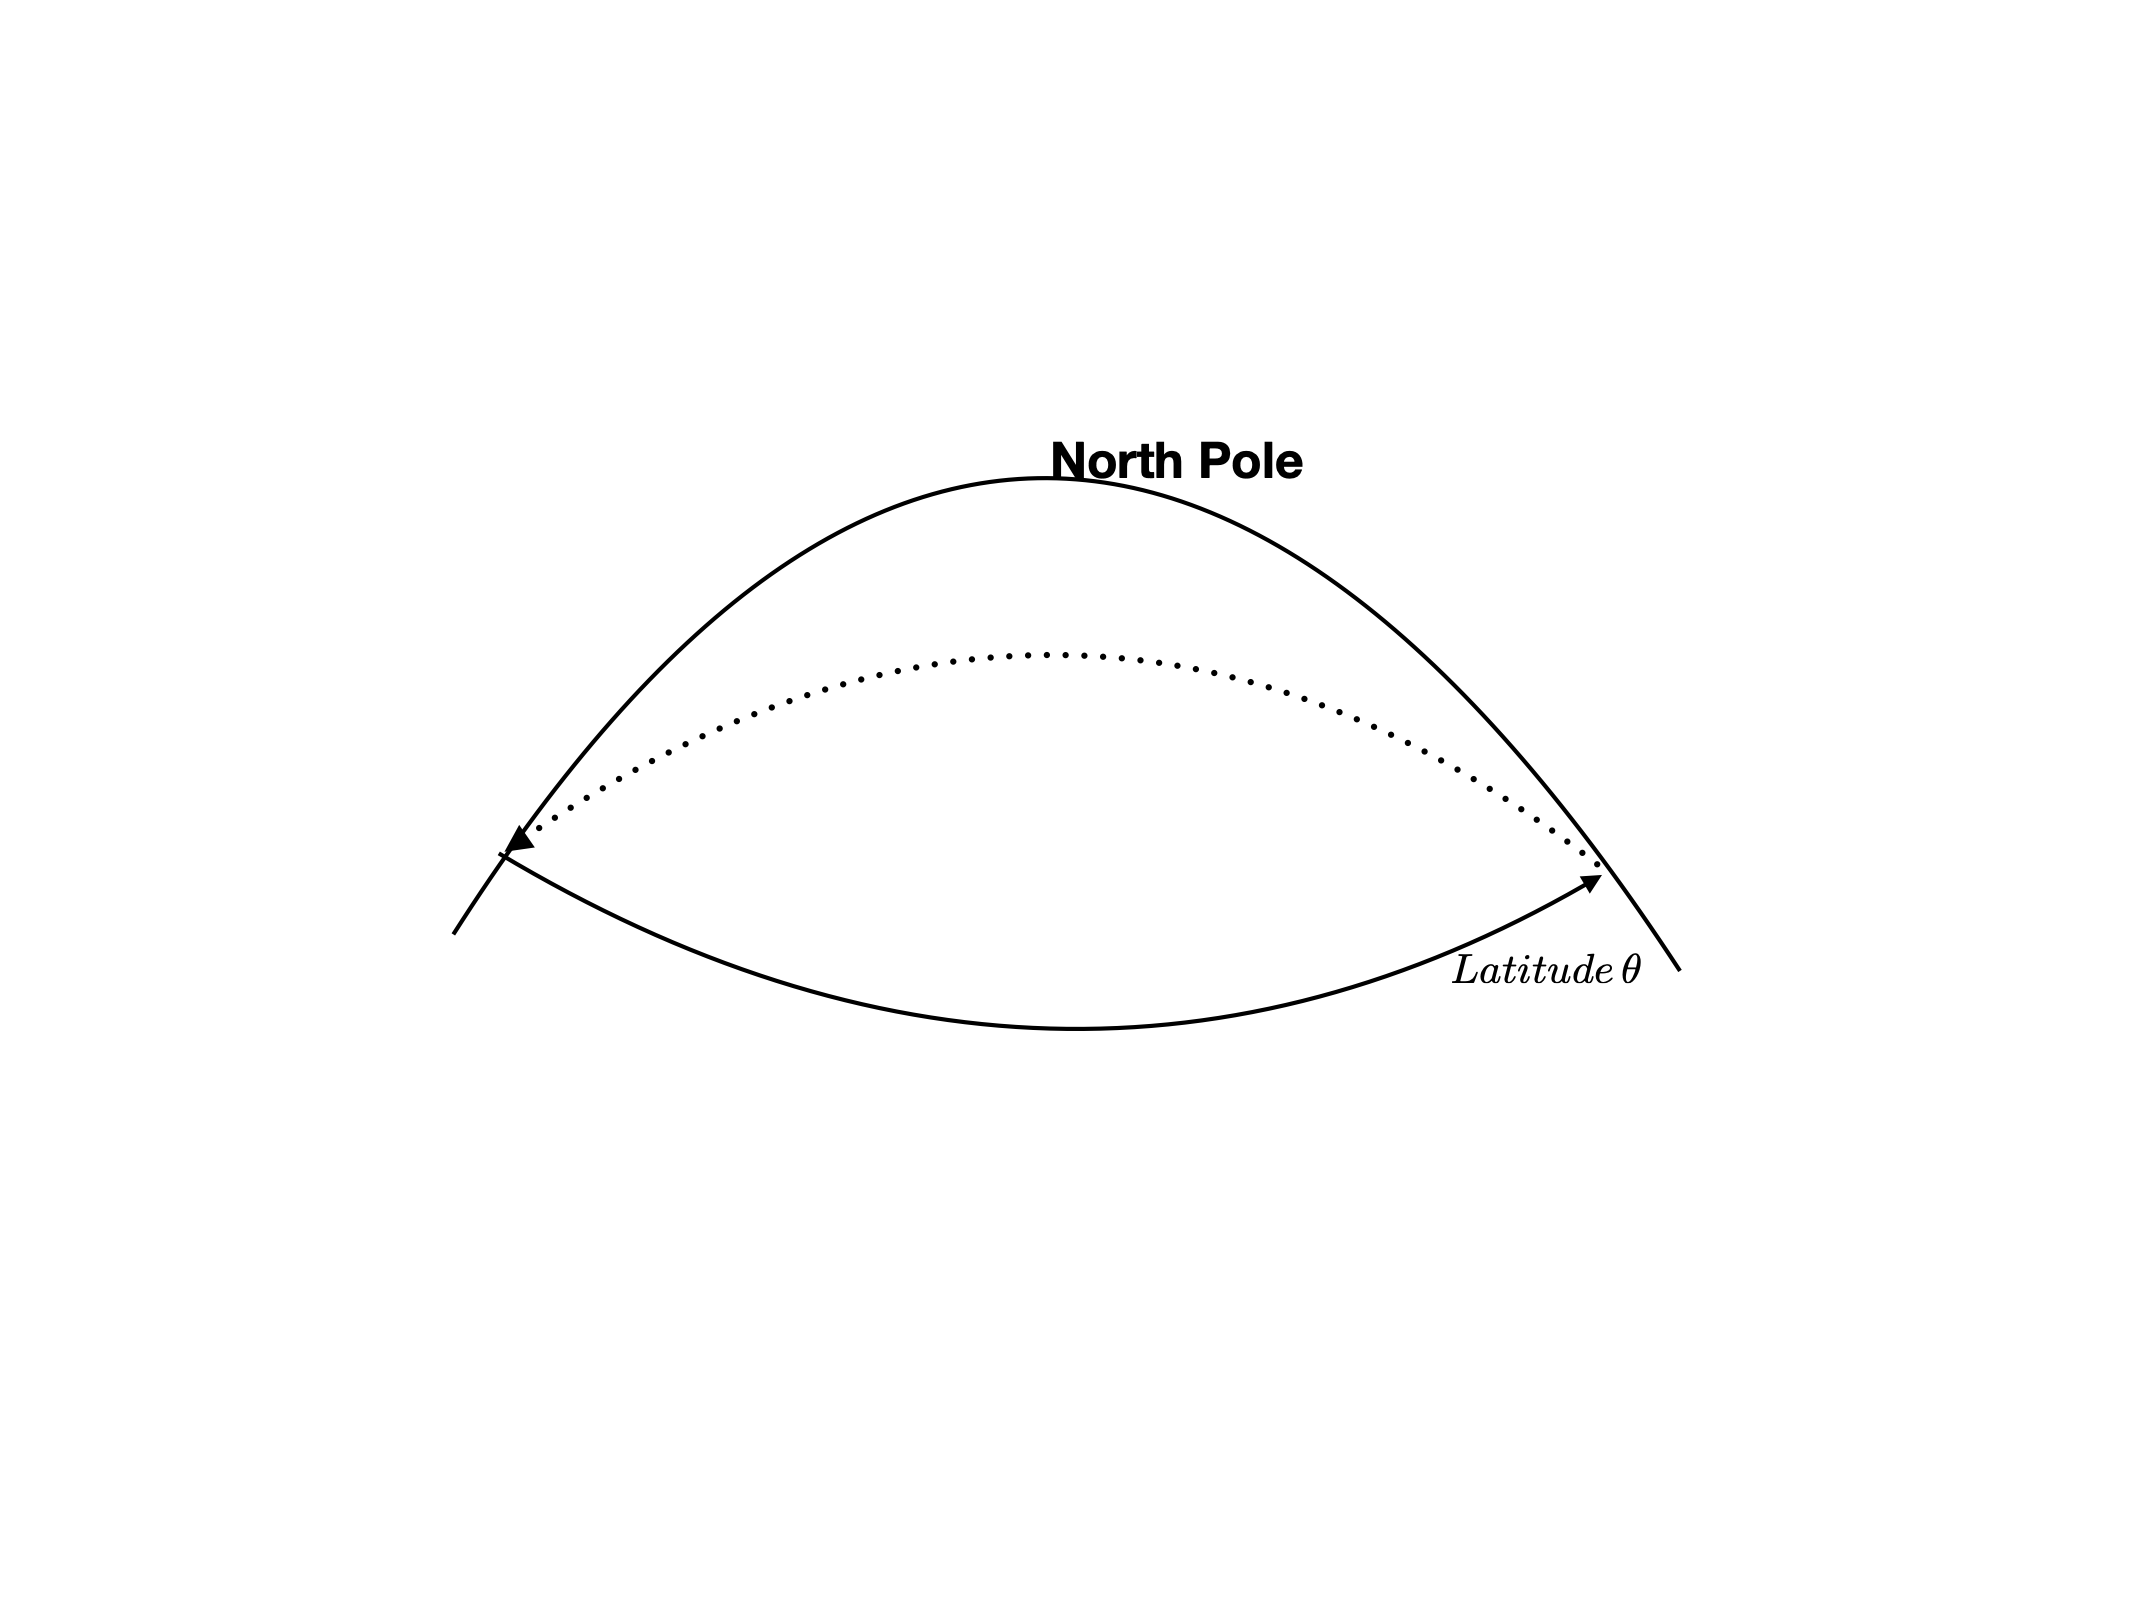
\includegraphics[width= .7 \textwidth]{figs/GD/polarcap.png}
\caption{}
\label{fig:}
\end{figure}

The circulation around the latitude circle is

{\[C=\int_0^{2\pi} u dx = \bar{u}2\pi \cos\theta\]}

however Stokes theorem offers a relation with vorticity

\[\int \mathbf{v}\cdot \mathbf{dl} = \int\nabla \times \mathbf{v}ds\]

that for the polar cap becomes

\[C=\int_{cap} \zeta \,ds = \int_\theta^{\pi/2}\, d\theta' \int_0^{2\pi} d\lambda\, a^2 \cos\theta' \zeta\]

From Eq \texttt{Ceq} we can also write

\[\frac{\partial \bar{u}}{\partial t} = \frac{1}{2\pi a\cos\theta}\frac{\partial C}{\partial t}\]

and so

\[\begin{aligned}
\frac{\partial \bar{u}}{\partial t} =\frac{1}{2\pi a\cos\theta}\int_\theta^{\pi/2}\, d\theta' \int_0^{2\pi}d\lambda\, a^2 \cos\theta' \frac{\partial \zeta}{\partial t} \\
=\frac{1}{2\pi a\cos\theta}\int_\theta^{\pi/2}\, d\theta' \int_0^{2\pi}d\lambda\, a^2 \cos\theta' \\
\left[ -\frac{1}{a \cos\theta}\frac{\partial }{\partial \lambda} (u\zeta) -\frac{1}{a \cos\theta}\frac{\partial }{\partial \theta}(\cos\theta v\zeta)\right]
\end{aligned}\]

the integrals are elementary and we end up with

\[\frac{\partial \bar{u}}{\partial t} = \overline{v \zeta}(\theta) =\overline{v'\zeta'}(\theta)\]

The zonal momentum into a polar cap can only change if there is a flux
of vorticity into the cap.

Exercise: Compute the zonal acceleration in a longitude channel

\subsection{The eddy equation}\label{the-eddy-equation}

Using the zonal mean we can split the vorticity equation on the
\(\beta\)-plane

\[\frac{\partial \zeta}{\partial t} = -\mathbf{v}\cdot\nabla(\zeta + f)\]

to obtain an equation for the zonally averaged part and the eddy
deviation

{\[\frac{\partial }{\partial t}(\bar{\zeta}+\zeta') = -(\bar{u}+u')\frac{\partial }{\partial x}(\bar{\zeta}+\zeta')-(\bar{v}+v')\frac{\partial }{\partial y}(\bar{\zeta}+\zeta'+f_0 +\beta y)\]}

zonally averaging both sides

{\[\frac{\partial \bar{\zeta}}{\partial t} = -\bar{u}\frac{\partial \bar{\zeta}}{\partial x}-\bar{v}\frac{\partial \bar{\zeta}}{\partial y}  -\beta\bar{v}- \frac{\partial }{\partial y}\overline{v'\zeta'}\]}

subtracting this equation (\texttt{zonzeta}) from the total
equation(\texttt{voreq}) we obtain the equation for the eddy component

{\[\frac{\partial \zeta'}{\partial t} = -\bar{u}\frac{\partial \zeta'}{\partial x} -v'\frac{\partial \bar{\zeta}}{\partial y}-\beta v'-\frac{\partial }{\partial x}(u'\zeta')-\frac{\partial }{\partial y}(v'\zeta'-\overline{v'\zeta'})\]}

If we can consider the perturbation as "small" in some sense, the
equation can be linearized to obtain

\[\begin{aligned}
\frac{\partial \bar{u}}{\partial t} &=\overline{v'\zeta'} \\  
\frac{\partial \zeta'}{\partial t} &= -\bar{u}\frac{\partial \zeta'}{\partial x} -v'( \frac{\partial \bar{\zeta}}{\partial y}+\beta)
\end{aligned}\]

Wer can define the absolute vorticity gradient \(\gamma\)

\[\gamma = \beta + \frac{\partial \bar{\zeta}}{\partial y} = \beta - \frac{\partial^{2} \bar{u}}{\partial y^{2}}\]

and the linearized equation becomes

{\[\frac{\partial \zeta'}{\partial t} = -\bar{u}\frac{\partial \zeta'}{\partial x} -\gamma v'\]}

This approximation are valid if the relative ratio of terms is small

\[\begin{aligned}
&\frac{O(\frac{\partial }{\partial x}u'\zeta'+ \frac{\partial }{\partial x} v'\zeta')}{O(\gamma v')} \approx \frac{\zeta'}{L\gamma} \\
&\frac{O(\frac{\partial }{\partial x}u'\zeta'+ \frac{\partial }{\partial x} v'\zeta')}{O(\bar{u}\frac{\partial \zeta'}{\partial x})} \approx \frac{u'}{U}
\end{aligned}\]

where \(U\) is the scale of the meridional variation of \(\bar{u}\).

\subsection{Enstrophy}\label{enstrophy}

The square of the vorticity \(\zeta^2\) is known as "enstrophy".
Multiplying Eq \texttt{vorlin} by \(\zeta'\) and averaging we get

{\[\frac{1}{2}\frac{\partial \overline{\zeta'^2}}{\partial t} = -\gamma\overline{v'\zeta'}\]}

The quantity \(\overline{\zeta'^2}\) is called "eddy enstrophy". It is a
square mean measure of the strength of the eddies, larger values of the
enstrophy indicate a more vigorous eddy field. The Eq \texttt{enslin}
tell us that the growth of the eddies is linked to the meridional flux
of eddy vorticity. If the \(\beta\) effect dominates and so
\(\gamma > 0\), then a negative (equatorward) vorticity flux indicate
growing eddies, whereas a positive (poleward) flux means decaying
eddies. To sustain eddy growth it is necessary am equatorward vorticity
flux.

Eq \texttt{enslin} has a companion nonlinear equation obtained
multiplying Eq \texttt{vornonlin} by \(\zeta'\) and averaging, namely

{\[\frac{1}{2}\frac{\partial \zeta'^2}{\partial t} = -\gamma\overline{v'\zeta'} -\frac{1}{2}\frac{\partial }{\partial y}\overline{v'\zeta'^2}\]}

so local growth of eddies can also be due to transport of enstrophy from
other regions. On the other hand we have seen in the previous section
that

{\[\frac{\partial \bar{u}}{\partial t} =\overline{v'\zeta'}=-\frac{1}{2\gamma}\frac{\partial }{\partial t}  \overline{\zeta'^2}\]}

this equation establishes a relation between the growth and decay of
eddies and the acceleration of the mean flow. Decaying eddies
(decreasing enstrophy) accelerate the zonal flow
(\(\frac{\partial \bar{u}}{\partial t}>0\)) , whereas growing eddies
will decelerate the zonal flow
(\(\frac{\partial \bar{u}}{\partial t}< 0\)).

\subsection{Steady flows}\label{steady-flows}

It is of particular interest the case of steady, inviscid flows. In this
case

\[\frac{1}{2}\frac{\partial \zeta'^2}{\partial t} = 0\]

and then Eq \texttt{enslin} is simply

\[\overline{v'\zeta'} = \frac{\partial }{\partial y}\overline{u'v'} = 0.\]

The vorticity flux is zero, but because it is linked to the divergence
of the momentum flux, the momentum flux itself \(\overline{u'v'}\) does
not need to be zero, This means that steady eddies still transport
momentum in a latitudinal direction.

This consideration show that then great importance must have the sources
and sinks of enstrophy. We can easily convinced ourselves that such
processes must exists since in their absence the motion would be steady,
so some processes must exist that generate enstrophy and some other
processes must exist that remove enstrophy so that an approximate
statistical balance is achieved, The simplest way to represent removal
processes is by dissipation terms in the equation, the processes
generating enstrophy are considerably more difficult and they cannot be
completely described in a 2-D flow, so we will simply indicate them as
an explicit forcing term. The new linear equation for the eddy vorticity
then can be written as

{\[\frac{\partial \zeta'}{\partial t} = -\bar{u}\frac{\partial \zeta'}{\partial x} -\gamma v'-\epsilon\zeta'+ \mathcal{F}\]}

It is possible to show that the dissipation term is not completely
arbitrary, but it is a representation of surface processes known as
"Ekman pumping", that is the way in which surface stresses act on the
internal flow. It will act not only on the eddies, but also on the
zonally averaged component. The forcing \(\mathcal{F}\) is often called
"stirring".

Multiplying by the eddy vorticity we obtain the version of Eq
\texttt{enslin} with sources and sinks

{\[\gamma\overline{v'\zeta'}= -\frac{1}{2}\frac{\partial \overline{\zeta'^2}}{\partial t} -\epsilon\overline{\zeta'^2}+\overline{\mathcal{F}\zeta'}\]}

or

{\[\frac{\partial \bar{u}}{\partial t} = -\frac{1}{2\gamma}\frac{\partial \overline{\zeta'^2}}{\partial t} -\frac{\epsilon}{\gamma}\overline{\zeta'^2}+\frac{1}{\gamma}\overline{\mathcal{F}\zeta'} -\epsilon\bar{u}\]}

This is an example of statistically steady, weakly stirred, dissipative
flow. Assume that \(\mathcal{F}\) is localized and otherwise zero, and
that \(\gamma \approx \beta\), i.e. the gradient of relative basic state
vorticity is small with respect the gradient of planetary vorticity.
From Eq \texttt{enssourcessinks} and \texttt{ubarsourcessinks} we then
have

\[\frac{\partial \bar{u}}{\partial t} = \overline{v'\zeta'} - \epsilon \bar{u}\]

Introducing now the time average, \(\{ \ \}\), we have a balance

\[\{ \bar{u}\} = \frac{1}{\epsilon}\{ \overline{v'\zeta'}\}\]

and using Eq \texttt{enssourcessinks} we also have

\[\{ \overline{v'\zeta'}\} = -\frac{\epsilon}{\beta}\{ \overline{\zeta'^2}\}\]

or

\[\{ \bar{u}\} = -\frac{1}{\beta}\{ \overline{\zeta'^2}\} ,\]

both equations are valid in the region where \(\mathcal{F}=0\).



\begin{figure}
\centering
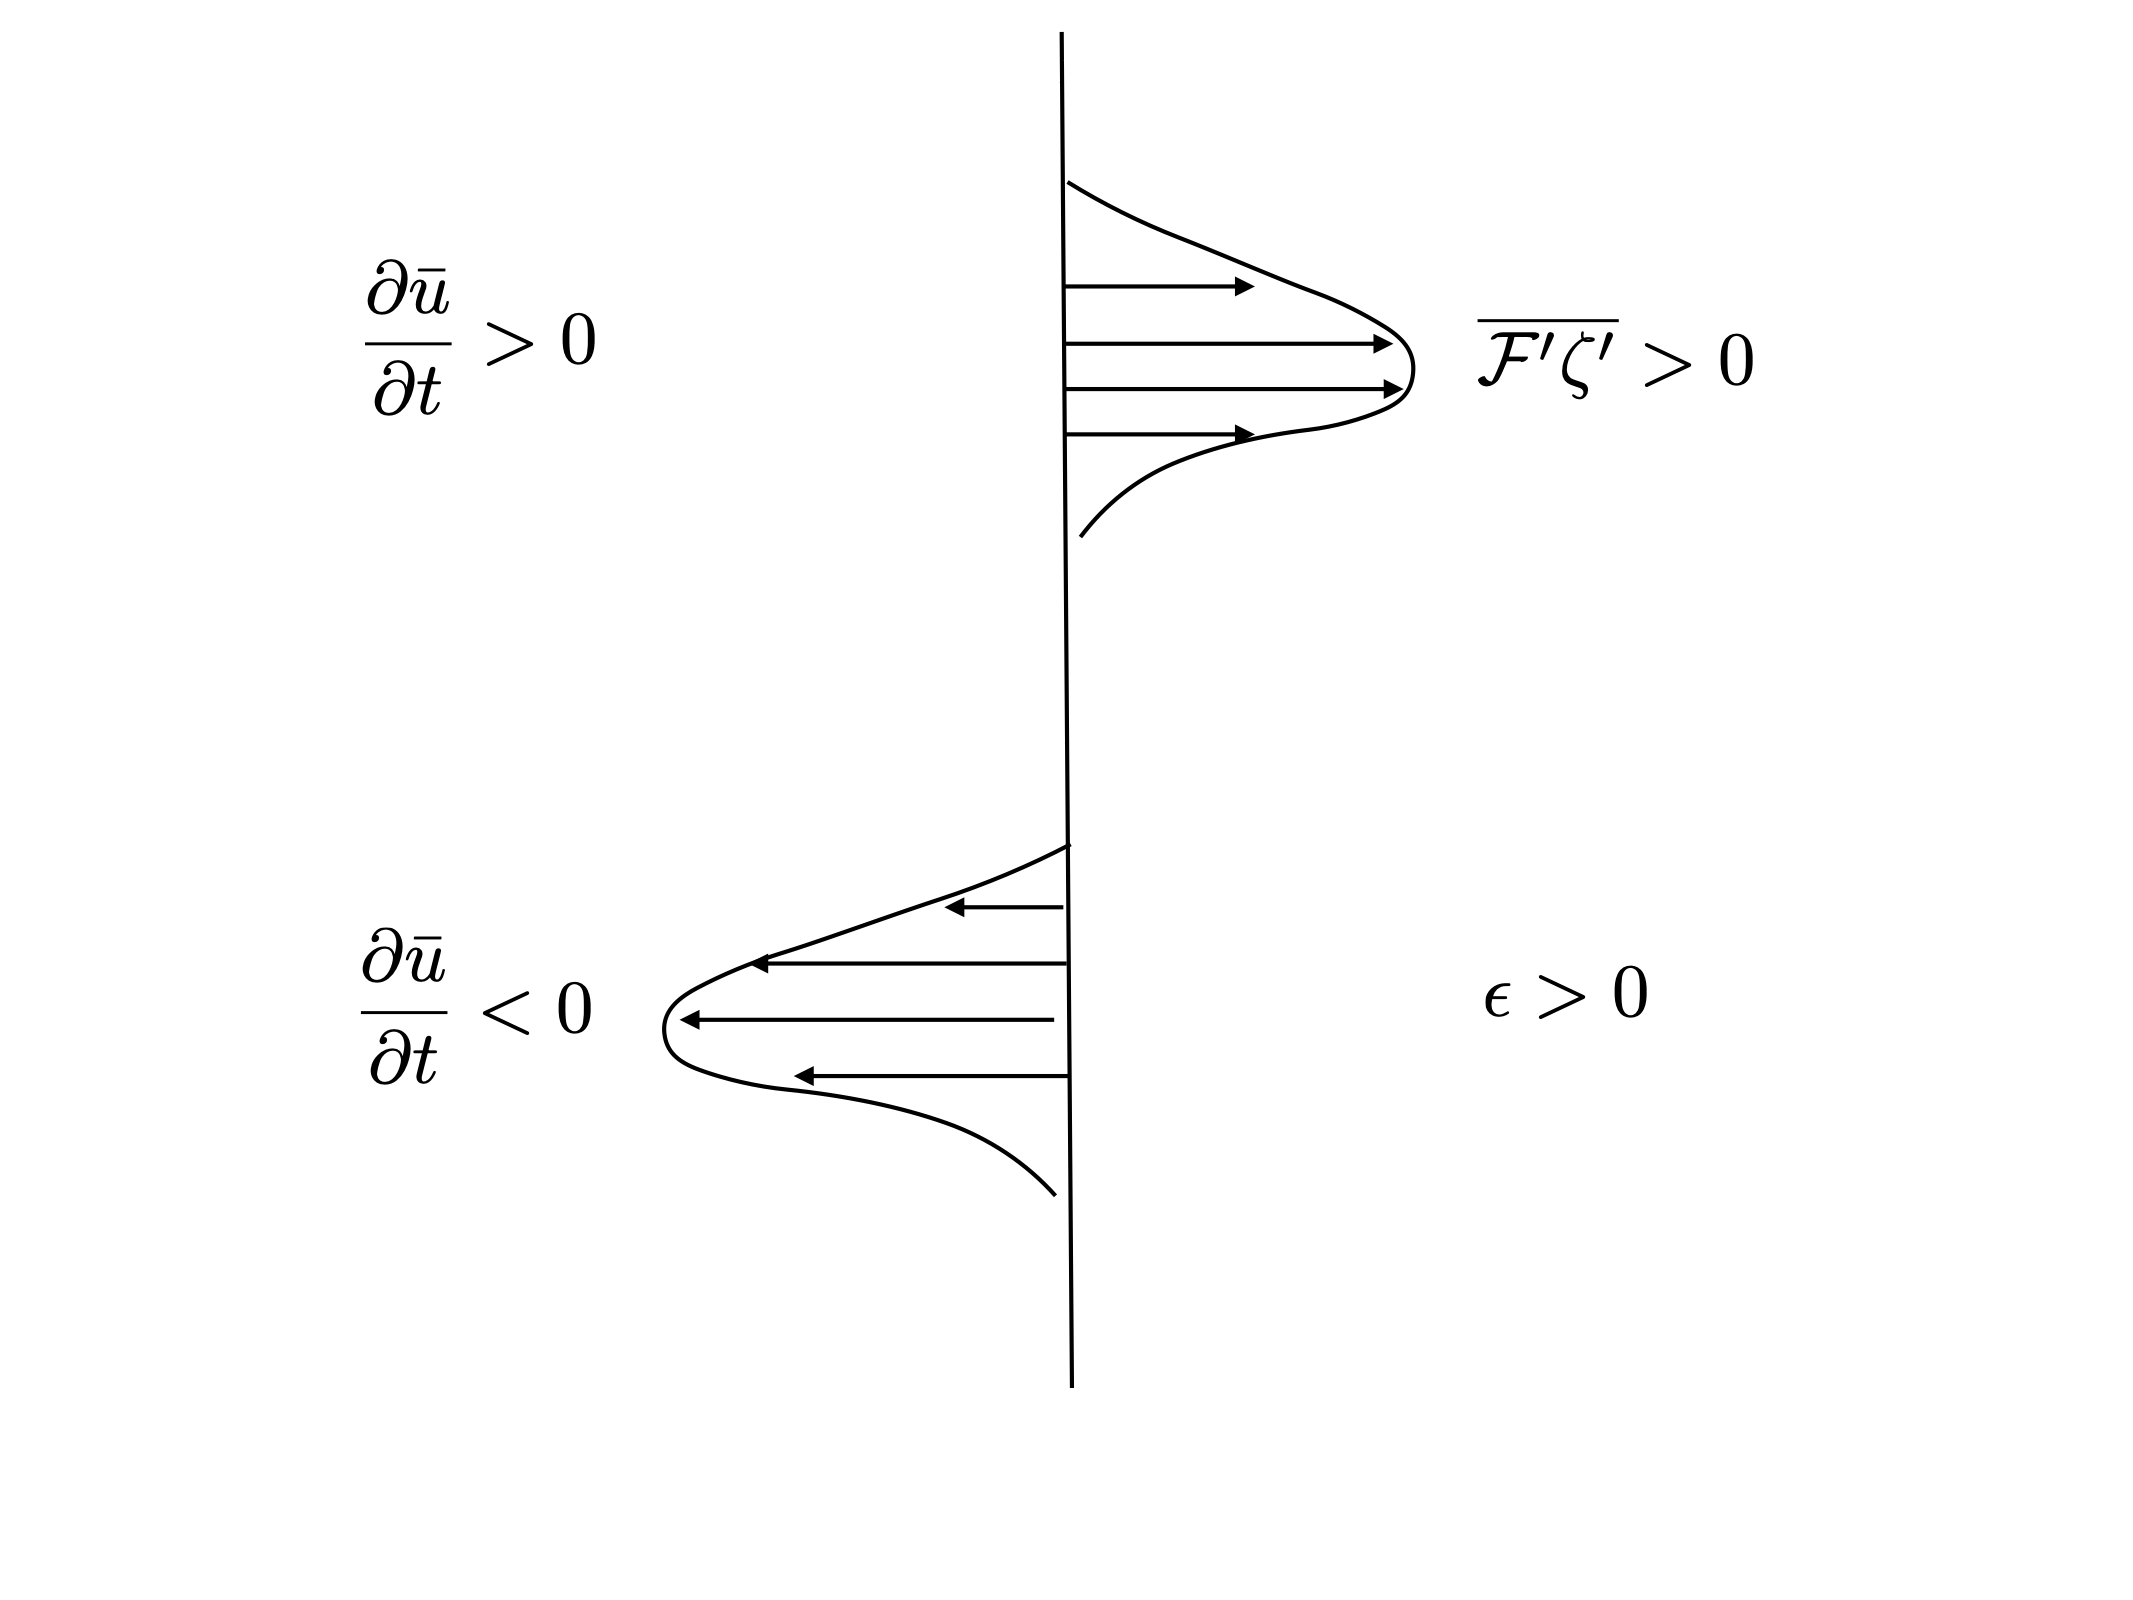
\includegraphics[width= .8 \textwidth]{figs/GD/ubarF.png}
\caption{}
\label{fig:}
\end{figure}

This relations point to the fact that in absence of forcing the presence
of eddies requires easterly in the zonal mean to respect the vorticity
balance. On the other hand angular momentum has to be conserved and this
means that westerly must be generated elsewhere and this can only happen
in the forcing region.

A more interesting case can be set up by assuming that also the
dissipation is acting only in a localized region. In this case something
must be carrying the momentum from one region to the other. The
Figure.\texttt{fig:2} shows a schematic of the situation. The region
were dissipation is acting forces a easterly tendency in the zonal flow
that can be compensated only by a westerly tendency in the forcing
region. Note the the forcing is actually realized by correlation terms
of the form \(\overline{\mathcal{F}'\zeta}\). These correlations are
always positive because a forcing of a certain sign generates a
vorticity eddy response of the same sign. Therefore for any
\(\mathcal{F} \neq 0\) the correlation terms for enstrophy are always
positive.
